\section{Problem statement}
This section will offer an overview of the key physics for the benefit
of readers from outside of experimental particle physics.

Particle colliders such as the LHC grant insight into physics by
creating heavy short lived particles that do not occur without a high energy collision
and only persist for a fraction of a second before decaying into lighter particles.
There is then a sequence of decays, known as a shower, before something
stable and long live enough to reach the detectors is created.
From the remnants of the decay that reach the detector we seek
to characterise the heavy particle created in the collision.
This is the raw data available to understand the event with.
In theory this is quite difficult and in practice it is also not easy.

The data pipeline can be seen as a whole in~\cite{Stoye_DeepCMS2018, Schramm:2291608}.
Evidence of the shower is gathered from multiple concentric detectors about the collision point, the primary components being the 
silicon tracker for charged particles and the calorimeter for neutral particles. 
These can be seen in figure~\ref{fig:lit_CMSdetector}.
\begin{figure}
    \centering
    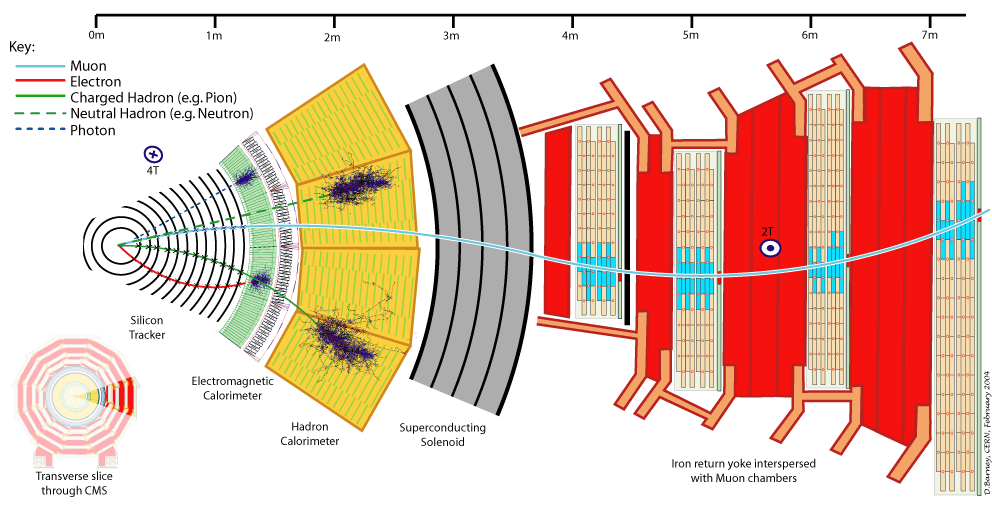
\includegraphics[width=0.8\textwidth]{images/lit_CMSdetector.png}
    \caption{The CMS detector has a concentric structure with each layer sensitive to a subset of possible particles.
             \cite{Stoye_DeepCMS2018}}
             % ADD could add more to this caption
    \label{fig:lit_CMSdetector}
\end{figure}
This data is essentially a series of energy deposits associated with three dimensional coordinates,
there is no time stamp available because the interaction occurs faster than the electronics can read out.
At this point the Particle Flow algorithm is used to reconstruct four vector tracks from the readings~\cite{Beaudette_particleFlow2013}.

There are often a great many particles in the shower by the time it reaches the detector,
attempting to cluster them by common origin,
into jets, is a key step in the reconstitution process.
It is particularly important for the identification and characterisation of quarks,
which will decay before the detector and have readily identified properties.
The majority of jets, however, come from gluons which radiate from the beam.
This clustering process will be considered in depth in later sections.

A good jet clustering algorithm needs to be infra-red and collinear safe~\cite[p.~10]{Salam2010TowardsJetography}
and it seeks to group the descendants of the quarks into exclusive clusters.
Thus the clustered jets can be used to estimate the kinematics of the quarks.
Jet clustering via novel methods is investigated in section~\ref{sec:JetClustering}.

Trimming may be used to remove `soft' radiation, that is products of beam radiation and lower energy interactions that occurred alongside the signal process.
Before the final stage considered here (tagging the jet) various preprocessing techniques may be applied to the jet and the tracks clustered in it.
Finally an algorithm will tag the jet, by estimating the identity of the particle that created it.

\subsection{Phenomonology}
In order to best develop tools to identify evidence of new physics it is important to establish what
a new physics is likely to appear.
There are many proposed, and as yet unobserved, ideas for new physics.
As mentioned in the introduction the 2HDM is the model considered throughout this work.

In its most general form the 2HDM adds \(6\) real parameters and \(4\) complex parameters.
These parameters can be further reduced by symmetry considerations.
Of the remaining parameter space the values of interest are constrained by two factors;
firstly the parameter choices must be such that it is reasonable that the particles created by the 2HDM
have not already been observed,
secondly the parameter choice need to be such that it is plausible we could differentiate
this model from the null hypothesis (the SM) using detectors available to us in the near future.

Applying these constraints refines the form of the signal that we design searches for to
one that is of greater interest.
This problem is addressed in more depth in section~\ref{sec:2HDM}.

\subsection{Simulation}

When developing tools, it is a great help to use data produced by Monte Carlo (MC) simulation.
Although this may be an imperfect representation of real particle behaviour 
it is a great advantage to be able to relate an observation to the high energy interaction that created it.
This MC truth information is very valuable in assessing the success of both jet clustering and 
jet formation techniques.

There are a variety of mature and well tested packages available for generating this data.
Specifically \lstinline{GEANT 4} \cite{agostinelli_geant4simulation2003} is used to simulate interactions between particles and the detector material.
\lstinline{POWHEG 2.0} \cite{alioli_powheg2010} and \lstinline{MadGraph5_aMC@NLO 2.2.2} \cite{alwall_madgraph2011} are used to generate signal events.
\lstinline{PYTHIA 8.2} \cite{sjostrand_pythia2015} is used to simulate the background, parton showering and hadronizsation.

\begin{figure}[htp]
    \begin{minipage}[c]{0.48\textwidth}
        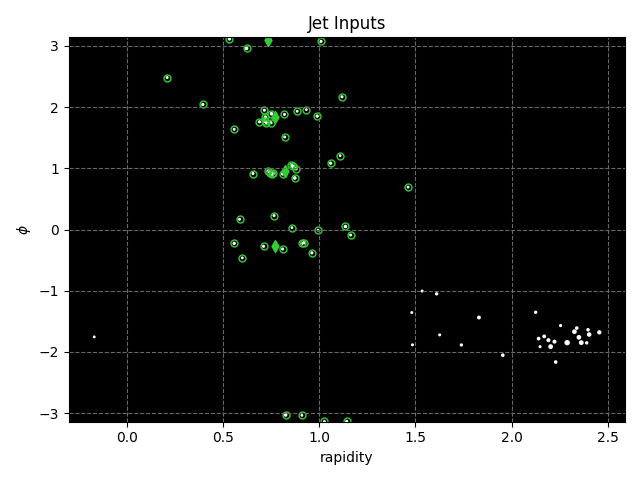
\includegraphics[width=1\textwidth]{graphics/truth_306.png}
        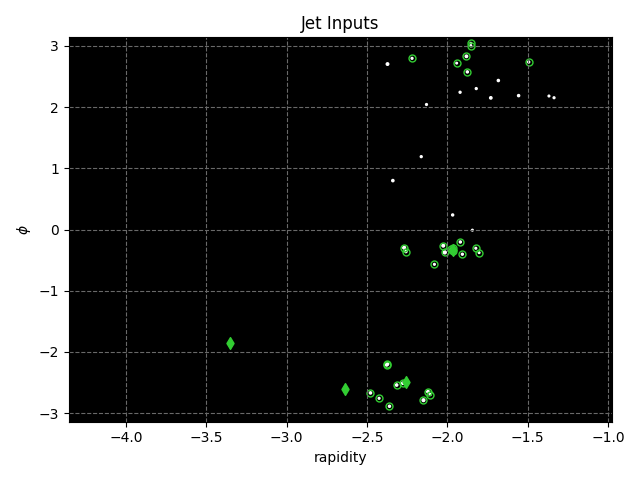
\includegraphics[width=1\textwidth]{graphics/truth_1936.png}
    \end{minipage}\hfill
    \begin{minipage}[c]{0.48\textwidth}
        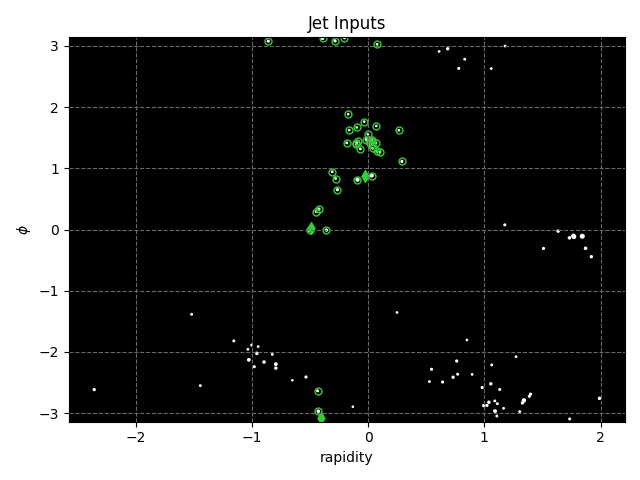
\includegraphics[width=1\textwidth]{graphics/truth_423.png}
        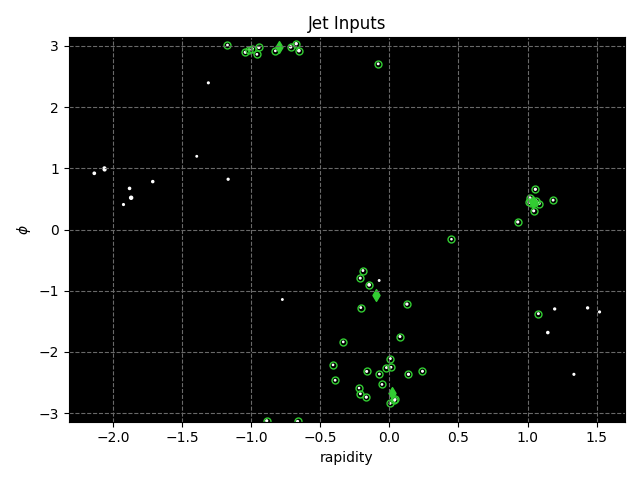
\includegraphics[width=1\textwidth]{graphics/truth_1378.png}
    \end{minipage}\hfill
    \caption{Some examples of events after particle cuts. 
             The images are each representations of the unrolled detector barrel.
             Each white dot is a particle that
             passes the cuts, thus is deemed detectable, and can be used for jet clustering.
             A green diamond indicates the location of the \bthing{quark}
             (not an input to clustering).
         A green circle indicates a descendant of the \bthing{quark}.} \label{fig:event_tracks_example}
\end{figure}    


For the purposes of jet physics, the next step is to identify
a particle in the MC truth as a tag particle.
In this study this tag particle is a \bthing{quark}.
The tag will decay before reaching the detector and 
jet physics aims to reconstruct it from its decay products.
The stable decay products that exist in the final state 
are termed here as `descendants'.
If these descendants have sufficient energy to be detectable and exist
at the right angle to meet the detector they are used as inputs for jet formation.
These are known as track cuts, and they stand in for the sensitivity of the detector.

Mixed in with the descendants are a number of other particles that have come from objects
that are not tags decaying.
In this study many of these are gluons radiated from the beam.
They form the background of the event and make jet formation
and identification more difficult.
Four examples of such events can be seen in fig~\ref{fig:event_tracks_example}.

These simulation tools are used throughout this work.
